\chapter{TINJAUAN PUSTAKA}
\label{chap:tinjauanpustaka}

% Ubah bagian-bagian berikut dengan isi dari tinjauan pustaka

Demi mendukung penelitian ini, terdapat beberapa jurnal penelitian terdahulu yang dijadikan sebagai pacuan dan referensi

\subsection{Non-Fungible Token (NFT): Overview, Evaluation, Opportunities and Challenges}
Qin Wang, bersama dengan dua rekan lainnya melakukan penelitian terhadap NFT yang dapat merubah pasar digital atau aset virtual. Dari hasil penelitian tersebut memberikan gambaran mendalam tentang teknologi NFT, potensinya, serta tantangan yang dihadapinya. Akan tetapi dalam jurnal penelitian tersebut tidak ada sangkut pautnya dengan pengimplementasian sistem blockchain dan smart contract yang sesuai judul dari penelitian, yaitu interoperabilitas dengan platform penyedia NFT lain.

\subsection{Blockchain technology for creative industries: Current state and research opportunities}
Nikhil Malik dan tiga rekan lainnya menuliskan jurnal penelitian terhadap teknologi blockchain yang dapat memiliki dampak kepada industri kreatif, seperti musik, desain grafis, permainan, dan software. Dalam jurnal tersebut, mereka menyoroti bagaimana NFT (non-fungible tokens) dan \emph{smart contracts} memberikan peluang menarik bagi industri kreatif. Meskipun teknologi ini telah menciptakan kegembiraan besar di pasar, di tengah-tengah kegemparan tersebut muncul nilai nyata bagi industri tersebut. Secara tradisional, para pencipta di industri kreatif seringkali harus bergantung pada perantara yang kuat untuk mendistribusikan dan mendapatkan keuntungan dari kreasi mereka. Namun, dengan adanya NFT dan \emph{smart contracts}, para pencipta kini dapat lebih dekat dengan konsumen/pembeli konten mereka. Selain itu, jurnal ini juga menggali fraksi pasar dan "biaya transaksi" yang dihadapi para pencipta ketika mendistribusikan konten kreatif mereka serta bagaimana \emph{smart contracts} dan NFT dapat mengubah dinamika pasar dengan mengurangi biaya-biaya tersebut. Namun, mereka juga menunjukkan keterbatasan dan tantangan yang mungkin dihadapi oleh para pencipta, pembeli, dan pasar dalam adopsi NFT dan \emph{smart contracts}.

\subsection{An Overview on Smart Contracts: Challenges, Advances and Platforms}
Penelitian tentang smart contract yang dilakukan oleh Zibin Zheng dan enam rekan lainnya ini menghasilkan pengetahuan berupa tinjauan mengenai teknologi smart contract yang mutakhir, tantangan dalam berbagai aspek pembuatan, penyebaran, eksekusi, dan penyelesaian \emph{smart contracts}, perbandingan beberapa platform smart contract utama, serta ulasan tentang teknologi smart contract dan blockchain. Tetapi dalam jurnal ini tentu saja terdapat beberapa kekurangan yang disampaikan oleh penulis yaitu meskipun smart contract berkembang pesat, masih ada banyak tantangan yang perlu diatasi.

\subsection{Blockchain for the metaverse: A Review}
Penelitian ini menyelidiki secara komprehensif peran dan dampak \emph{blockchain} untuk dasar dan pengembangan aplikasi dan layanan di metaverse. Jurnal yang ditulis oleh Thien Gadekallu dan 7 peneliti lain ini memberikan gambaran beserta dengan pengetahuan mengenai konsep dasar \emph{blockchain} dan metaverse. Dalam jurnal ini pembaca dapat mengetahui tantangan yang perlu ditangani, seperti algoritma konsensus, manajemen jaringan, dan interoperabilitas \emph{blockchain}. 

\section{Dasar Teori}

\subsection{\emph{Blockchain}}
\emph{Blockchain} merupakan teknologi basis data terdistribusi yang mengizinkan data disimpan dalam serangkaian blok yang terkoneksi. Tiap blok mengandung rangkaian transaksi yang sudah divalidasi, dan setiap penambahan blok baru ke dalam rantai menjamin keabadian dan ketidakmampuan modifikasi dari transaksi yang tercatat. Fitur keamanan dan keterbukaan menjadi ciri khas \emph{blockchain} karena setiap transaksi divalidasi oleh jaringan partisipan dan tercatat dalam sebuah rantai yang tak bisa dimodifikasi. Berkat struktur terdesentralisasinya, \emph{blockchain} menawarkan ketahanan terhadap modifikasi atau upaya peretasan, sehingga memastikan keutuhan dan keotentikan data. \cite{Tjokrosetio22}

\emph{Blockchain} menyediakan catatan keuangan yang aman dan disimpan secara terdesentralisasi. Fungsi ini memiliki dampak penting bagi pemasaran. Berdasarkan fungsi ini, muncul dua teknologi yang relevan bagi industri kreatif, yaitu \emph{smart contract} dan non-fungible tokens (NFT). NFT mengidentifikasi karya seni unik dan mencatat kepemilikannya di \emph{blockchain}. \emph{Smart contract} adalah program yang disimpan di \emph{blockchain} yang otomatis menjalankan perjanjian saat kondisi yang telah ditentukan terpenuhi. \emph{Smart contract} dapat digunakan untuk menetapkan aturan penjualan, penggunaan, dan lisensi NFT \cite{Malik2023}.

Blockchain merupakan teknologi yang revolusioner dalam menyimpan dan mengelola data secara terdesentralisasi melalui jaringan komputer yang saling terhubung. Setiap blok dalam blockchain berisi batch transaksi yang telah divalidasi oleh partisipan jaringan, yang kemudian secara kronologis ditambahkan ke dalam rantai blok sebelumnya, menciptakan catatan permanen yang tidak dapat diubah atau dihapus. Keamanan ini diperkuat melalui penggunaan kriptografi untuk mengamankan transaksi dan memastikan integritas dan autentisitas data. Sebagai sebuah sistem yang terdesentralisasi, blockchain mengurangi risiko manipulasi data dan penyalahgunaan kekuasaan, karena tidak ada satu entitas pun yang dapat mengontrol seluruh jaringan.

Dalam konteks pemasaran dan industri kreatif, dua aplikasi blockchain yang sangat penting adalah \emph{smart contract} dan \emph{Non-Fungible Tokens} (NFT). \emph{Smart contract} adalah protokol yang memungkinkan kontrak otomatis dijalankan ketika kondisi yang telah disepakati terpenuhi tanpa memerlukan intervensi pihak ketiga. NFT, di sisi lain, adalah token unik yang tidak dapat dipertukarkan satu sama lain dan sering digunakan untuk mewakili kepemilikan atas aset digital unik seperti karya seni, koleksi digital, dan lebih banyak lagi, semua tercatat di blockchain. Dengan demikian, blockchain tidak hanya berfungsi sebagai teknologi yang mendukung transaksi keuangan tetapi juga memainkan peran penting dalam mengotomatisasi dan mengamankan transaksi digital dalam ekonomi digital yang lebih luas.

\subsection{Mekanisme \emph{Blockchain}}
\emph{Blockchain} merupakan teknologi yang mengubah cara data disimpan dan dikelola dalam jaringan yang terdesentralisasi. Berbeda dari sistem penyimpanan data tradisional yang mengandalkan server pusat, \emph{blockchain} menyimpan data dalam rangkaian \emph{blok} yang dihubungkan satu sama lain melalui \emph{hash} kriptografi. Setiap \emph{blok} baru yang ditambahkan mengandung tanda tangan digital yang tidak hanya melindungi integritas data tetapi juga memastikan bahwa data tersebut tidak dapat diubah setelah dikonfirmasi oleh jaringan.

\begin{figure} [H] \centering
    % Nama dari file gambar yang diinputkan
    \frame{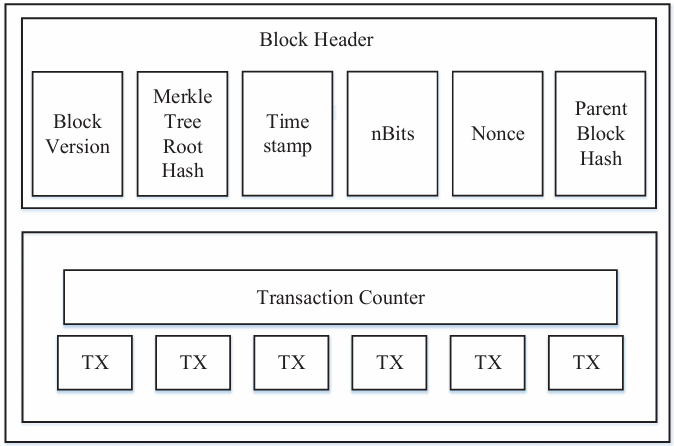
\includegraphics[scale=0.75]{gambar/blockchain_sequence.png}}
    % Keterangan gambar yang diinputkan
    \caption{Struktur dari \emph{Blockchain} \cite{Zheng2020}}
    % Label referensi dari gambar yang diinputkan
    \label{fig:blockchain}
    \end{figure}

Karakteristik utama dari \emph{blockchain} mencakup desentralisasi, ketahanan, \emph{anonimitas}, dan \emph{auditabilitas}. Dengan desentralisasi, \emph{blockchain} mengeliminasi kebutuhan akan otoritas pusat, yang mengurangi biaya dan meningkatkan efisiensi. Ketahanan \emph{blockchain} menjamin bahwa setelah data dimasukkan, data tersebut hampir mustahil dihapus atau dimodifikasi. Ini memberikan tingkat keamanan yang tinggi yang sangat cocok untuk transaksi keuangan dan aplikasi lain yang memerlukan tingkat kepercayaan tinggi.

Dalam konteks \emph{anonimitas}, \emph{blockchain} memungkinkan pengguna untuk berinteraksi di dalam jaringan menggunakan alamat yang dihasilkan secara acak yang tidak mengungkapkan identitas sebenarnya dari pengguna. Namun, ini tidak menjamin privasi sepenuhnya karena transaksi dan saldo tetap terlihat publik di jaringan. Oleh karena itu, meskipun pengguna beroperasi dalam \emph{anonimitas}, aktivitas mereka di dalam jaringan masih bisa dilacak jika ada kebutuhan.

\emph{Auditabilitas} \emph{blockchain} memungkinkan semua transaksi yang tercatat diverifikasi dan ditelusuri kembali oleh siapa pun di jaringan. Ini mencegah penipuan dan memastikan bahwa semua pengguna mematuhi aturan yang ditetapkan oleh protokol \emph{blockchain}.

Dengan menggabungkan semua karakteristik ini, \emph{blockchain} menawarkan solusi yang kuat dan transparan untuk berbagai kebutuhan aplikasi, dari keuangan hingga rantai pasok, yang memanfaatkan kekuatan teknologi desentralisasi untuk meningkatkan keamanan dan efisiensi operasional. \cite{Zheng2020}

    \begin{figure} [H] \centering
    % Nama dari file gambar yang diinputkan
    \frame{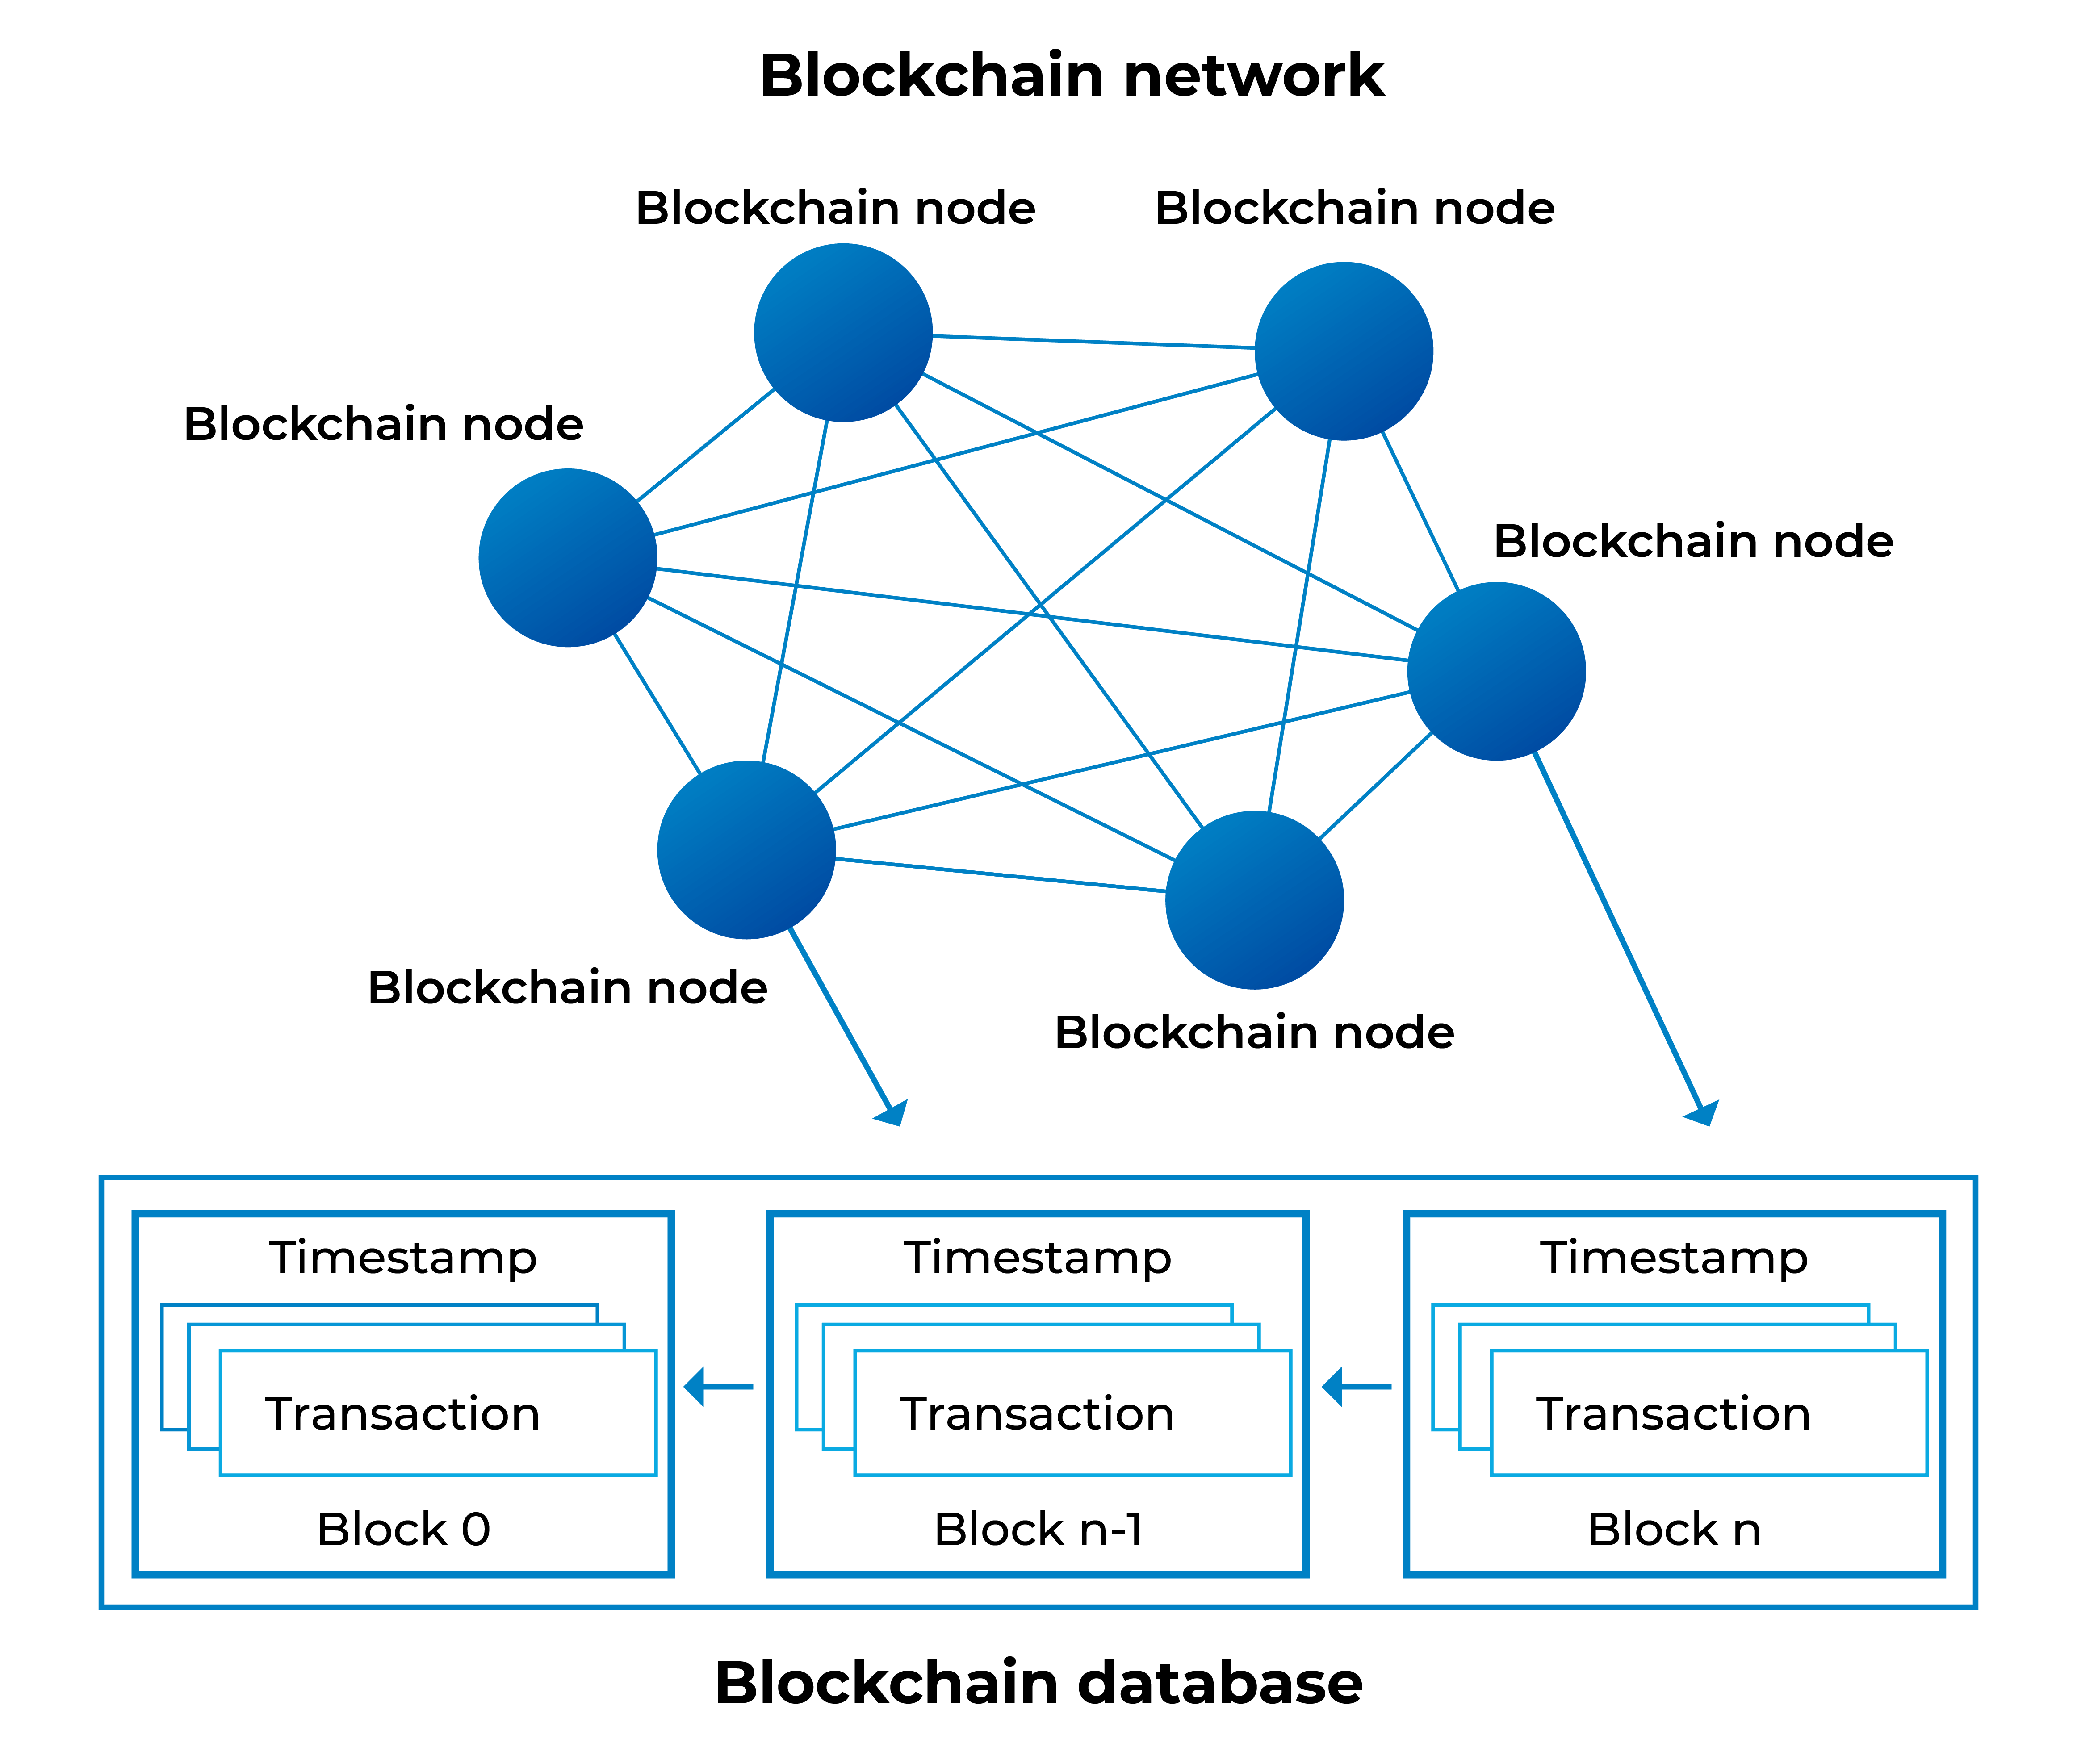
\includegraphics[scale=0.075]{gambar/topology_blockchain.png}}
    % Keterangan gambar yang diinputkan
    \caption{Topology Blockchain \cite{Zheng2020}}
    % Label referensi dari gambar yang diinputkan
    \label{fig:blockchain}
    \end{figure}

    Dalam blockchain, tiap blok data mengandung informasi transaksi yang divalidasi dan dicatatkan dalam timestamp yang spesifik. Sebuah blok baru (disebut sebagai "Block n") ditambahkan ke dalam rantai blok hanya setelah berhasil divalidasi dan disetujui oleh jaringan, dan setiap blok baru mengandung referensi kriptografis ke blok sebelumnya (disebut sebagai "Block n-1"), membentuk rantai data yang konsisten dan tidak terputus.

    Struktur ini memastikan integritas data dan ketahanan terhadap upaya manipulasi karena setiap blok baru yang ditambahkan memerlukan konsensus dari mayoritas node dalam jaringan. Keunikan blockchain ini juga terletak pada kemampuannya untuk menyimpan data secara terdesentralisasi, berbeda dengan sistem database tradisional yang menggunakan server pusat. Kemampuan ini memberikan keamanan tambahan serta transparansi karena setiap partisipan dalam jaringan memiliki akses ke seluruh riwayat transaksi yang tidak bisa diubah atau dihapus.

\subsection{Ethereum}

Ethereum, sebuah platform \emph{blockchain} terdesentralisasi yang diperkenalkan oleh Vitalik Buterin pada tahun 2013, memfasilitasi pembuatan dan pelaksanaan aplikasi terdistribusi, dikenal sebagai kontrak pintar (\emph{smart contract}). Platform ini, yang memajukan ide \emph{blockchain} , mengizinkan eksekusi kode pemrograman tingkat lanjut langsung dalam sistem \emph{blockchain}-nya, menggunakan mata uang digital bernama Ether (ETH) untuk melangsungkan transaksi dan mengoperasikan \emph{smart contract}. Ether (ETH), mata uang digital dalam jaringan Ethereum, tidak hanya berfungsi sebagai alat pembayaran tetapi juga diperlukan untuk menjalankan \emph{smart contract}. Setiap kali \emph{smart contract} dijalankan, pemiliknya harus membayar biaya dalam Ether, dikenal sebagai biaya \emph{gas}, yang mencegah spam dan memastikan penggunaan sumber daya jaringan yang efisien. Fitur penting Ethereum adalah kemampuan Turing-completeness, yang memungkinkannya menjalankan berbagai aplikasi terdistribusi. Ini memberi pengembang kebebasan untuk menciptakan aplikasi yang lebih kompleks dan beragam, mulai dari permainan hingga pasar digital, sistem keuangan terdesentralisasi, identitas digital, dan banyak lagi. Selain itu, Ethereum memungkinkan penciptaan token ERC-20, memberikan pengguna kemampuan untuk membuat dan mengelola token mereka sendiri di ekosistem Ethereum. Token ini digunakan untuk berbagai tujuan, termasuk dalam Initial Coin Offering (ICO) untuk penggalangan dana proyek baru, atau sebagai aset digital yang dapat ditukar di bursa kripto \cite{Antonopoulos2018}.

\subsection{\emph{Ethereum Virtual Machine} (EVM)}

Ethereum Virtual Machine (EVM) adalah komponen kunci yang memungkinkan Ethereum untuk berfungsi sebagai platform bagi \emph{smart contracts}. Setiap komputer yang terhubung ke jaringan Ethereum memiliki EVM yang memungkinkannya untuk menjalankan kode yang sama, memastikan bahwa setiap smart contract menghasilkan output yang konsisten di seluruh jaringan. EVM bersifat Turing lengkap, yang berarti ia mampu mengeksekusi berbagai instruksi yang diberikan kepadanya, asalkan instruksi tersebut disampaikan dalam format bytecode yang ia mengerti. Pengembang biasanya menulis smart contract dalam bahasa yang lebih aksesibel seperti Solidity atau Vyper sebelum mengompilasinya menjadi bytecode untuk EVM. EVM tidak hanya menjalankan kode ini, tetapi juga mengawasi dan memelihara keadaan semua informasi di \emph{blockchain} Ethereum, termasuk saldo akun dan data yang disimpan oleh \emph{smart contracts}. Untuk menjaga kestabilan dan mencegah penyalahgunaan sistem, EVM menggunakan sistem biaya yang dikenal sebagai gas, yang membatasi jumlah sumber daya yang dapat dikonsumsi oleh setiap smart contract. Dengan demikian, EVM adalah mesin yang kuat dan fleksibel yang memungkinkan berjalannya aplikasi terdesentralisasi yang aman dan tidak dapat diubah dalam lingkup Ethereum. \cite{Dannen2017}

\subsection{Token}
Token secara umum didefinisikan sebagai unit nilai digital yang tercatat pada \emph{blockchain}. Dalam ekosistem \emph{blockchain}, token dapat diklasifikasikan ke dalam beragam kategori berdasarkan ciri khasnya. Dua klasifikasi utama token dalam \emph{blockchain} adalah token berbasis klaim dan token berbasis objek. Token berbasis objek memiliki nilai intrinsik, biasanya ditentukan oleh dinamika permintaan dan penawaran. Sebaliknya, \emph{token} berbasis klaim, yang sering dikenal sebagai \emph{stablecoin}, dirancang untuk mempertahankan nilai stabilnya, seringkali dengan mengaitkannya dengan nilai aset likuid \cite{Freni2022}. 
Di dalam \emph{blockchain} Ethereum, terdapat standar tertentu yang harus diikuti agar token dapat berinteraksi dengan berbagai aplikasi desentralisasi yang ada di dalam jaringan. Beberapa standar yang telah ditetapkan untuk pengembangan di \emph{blockchain} Ethereum meliputi:
\begin{itemize}
    \item ERC-20, \emph{interface} standar untuk fungible token, di mana setiap unit token memiliki nilai yang sama, memungkinkan pertukaran dalam jumlah yang setara.
    \item ERC-721, \emph{interface} standar untuk non-fungible token, di mana setiap token bersifat unik dan memiliki nilai yang berbeda.
    \item ERC-1155, \emph{interface} standar yang berlaku untuk baik fungible maupun non-fungible token.
    \item ERC-1633, \emph{interface} standar untuk memungkinkan pembagian kepemilikan NFT, sehingga satu NFT bisa dimiliki oleh lebih dari satu pihak.
    \item ERC-4907, \emph{interface} standar yang memperkenalkan peran baru dalam NFT, yaitu pemilik (owner) dan pengguna (user) yang memiliki akses terbatas terhadap NFT tersebut selama jangka waktu tertentu.
\end{itemize}

\subsection{\emph{Non-Fungible Token} (NFT)}

Non-Fungible Token atau NFT merupakan varian mata uang kripto yang berasal dari \emph{smart contract} di Ethereum. NFT pertama kali diperkenalkan melalui Ethereum Improvement Proposals (EIP)-721 dan diperluas melalui EIP-1155. NFT membedakan diri dari mata uang kripto konvensional, misalnya Bitcoin. Jika Bitcoin memiliki koin-koin yang sama dan identik, NFT justru dikenal dengan keunikannya yang tidak bisa digantikan atau ditukar secara setara, menjadikannya alat identifikasi yang unik. Menggunakan NFT di dalam \emph{smart contract} Ethereum memungkinkan pencipta untuk memvalidasi keberadaan dan kepemilikan aset digital seperti video, gambar, karya seni, tiket, dan sebagainya. Pencipta bahkan dapat mendapatkan royalti setiap kali aset mereka diperdagangkan di pasar NFT atau melalui transaksi peer-to-peer. Berkat fitur transaksinya yang transparan, likuiditas tinggi, serta kemudahan integrasi, NFT menjadi alat yang efektif dalam melindungi hak kekayaan intelektual. Walaupun esensinya NFT hanyalah kode, namun kode tersebut memiliki nilai tersendiri bagi pembeli karena kelangkaannya, menjadikannya alat penting dalam menetapkan harga bagi produk dengan hak kekayaan intelektual di dunia digital \cite{Wang2021}.

\subsection{\emph{Minting}}
Dalam konteks \emph{smart contracts}, "minting token" mengacu pada proses pembuatan dan pelepasan \emph{token} baru dalam jaringan \emph{blockchain}. Proses ini krusial dalam mengembangkan ekosistem \emph{token} untuk aplikasi dan platform berbasis \emph{blockchain}. Minting token umumnya dilakukan melalui \emph{smart contracts} yang mengadopsi standar \emph{token} seperti ERC-20 atau ERC-721 di Ethereum. \emph{Smart contracts} tersebut memiliki fungsi khusus untuk menghasilkan \emph{token} baru dan menetapkan karakteristiknya, biasanya dilakukan oleh pemilik kontrak atau entitas berwenang lainnya. Selama minting, catatan transaksi yang merekam pembuatan dan penerbitan \emph{token} baru juga direkam secara permanen dalam \emph{blockchain}, menjamin keaslian dan riwayat kepemilikan \emph{token}. Informasi ini dapat diakses dan diverifikasi oleh semua peserta jaringan, menawarkan transparansi dan kepercayaan dalam ekosistem \emph{token}. 

Untuk \emph{smart contracts} berstandar ERC-20, fungsi mint atau fungsi serupa digunakan untuk menghasilkan \emph{token} baru. Fungsi ini memerlukan parameter seperti jumlah \emph{token} yang akan dibuat dan alamat pemilik \emph{token} pertama. Setelah dipanggil, kontrak akan menghasilkan \emph{token} baru dan menetapkan ciri-cirinya seperti simbol, nama, total pasokan, dan pemilik awal. Dalam kontrak pintar ERC-721, proses minting melibatkan fungsi yang mirip. Namun, dalam konteks \emph{token} non-fungible (NFT), tiap \emph{token} memiliki identitas dan karakteristik unik. Proses minting di ERC-721 melibatkan penetapan atribut spesifik untuk setiap \emph{token}, termasuk metadata yang menggambarkan aset yang direpresentasikan oleh \emph{token}. 

Proses minting \emph{token} memiliki dampak luas dalam ekosistem \emph{blockchain}, memungkinkan penciptaan \emph{token} baru untuk berbagai aplikasi seperti keuangan, pasar NFT, game \emph{blockchain}, identitas digital, dan lainnya. Minting \emph{token} membantu pengembang menciptakan ekonomi digital yang dinamis dan inovatif di atas teknologi \emph{blockchain}. 

\subsection{\emph{Smart Contracts}}
Smart Contract adalah protokol transaksi yang diotomatisasi, yang melaksanakan syarat-syarat dalam suatu perjanjian. Ketika suatu kondisi tertentu dipenuhi, klausul dalam \emph{smart contracts} akan otomatis dieksekusi. Smart contract dibuat di atas blockchain, di mana setiap eksekusi pernyataan kontrak dicatat sebagai transaksi yang tidak dapat diubah. Dalam pengembangannya, pengembang dapat menentukan izin akses untuk setiap fungsi dalam kontrak. Misalnya, jika seseorang melanggar kontrak, sanksi yang ditentukan dalam kontrak akan otomatis dikenakan. Smart Contract merupakan kemajuan penting dalam teknologi blockchain \cite{Zheng2020}.

Smart Contract dapat dikembangkan dan diterapkan di berbagai platform \emph{blockchain} (misalnya, NXT, Ethereum, dan Hyperledger Fabric). Beberapa platform menawarkan fitur khusus untuk mengembangkan \emph{smart contracts}, termasuk bahasa pemrograman, eksekusi kode, dan tingkat keamanan. Beberapa platform mendukung bahasa pemrograman tingkat tinggi untuk mengembangkan \emph{smart contracts} \cite{Khan2021}.

\subsection{\emph{InterPlanetary File System} (IPFS)}
\emph{InterPlanetary File System } (IPFS) adalah platform berbagi file yang desentralisasi, dirancang untuk menyimpan dan mengakses file, website, aplikasi, dan data dengan cara yang lebih efisien dan tidak bergantung pada server tunggal. IPFS menggunakan teknologi \emph{hash} kriptografi untuk mengidentifikasi setiap potongan data secara unik, sehingga memudahkan verifikasi dan pengambilan data tanpa perlu mengandalkan lokasi pusat. Selain itu, IPFS menggabungkan file menjadi unit yang lebih besar menggunakan grafik yang diarahkan dan tidak berulang, yang dikenal sebagai Merkle DAGs. Ini memungkinkan distribusi dan penyimpanan data secara efisien di banyak komputer.

IPFS mengurangi redundansi dan meningkatkan kecepatan dengan menyimpan data hanya sekali namun membuatnya dapat diakses dari banyak komputer yang memiliki salinan atau bagian dari data tersebut. Ketika file diunggah ke IPFS, file tersebut dipecah menjadi blok-blok kecil yang masing-masing diidentifikasi melalui \emph{hash} kriptografi. Jika dua file atau bagian dari file mengandung data yang sama, mereka akan berbagi blok yang sama di IPFS, menghemat ruang dan mengurangi duplikasi.

Keunggulan terbesar IPFS adalah kemampuannya untuk membuat web lebih tahan terhadap kegagalan, karena menghilangkan titik kegagalan tunggal dan memberikan distribusi yang lebih luas dari konten. Hal ini sangat berharga dalam kasus sensor atau infrastruktur internet yang terbatas. Dengan menyimpan data di banyak tempat, akses ke informasi bisa menjadi lebih cepat dan lebih andal, meningkatkan pengalaman pengguna global terhadap internet yang lebih terdesentralisasi. \cite{Steichen18}.

\subsection{Web 3.0}
Web 3.0 merupakan era baru dalam perkembangan internet, dikenal sebagai internet desentralisasi atau semantic web. Konsep ini muncul sebagai respons terhadap kekuasaan terpusat yang dimiliki oleh raksasa teknologi dalam mengelola data di Web 2.0, yang sering kali menimbulkan masalah privasi dan monopoli data. Web 3.0 memanfaatkan teknologi blockchain untuk memberikan kontrol lebih besar kepada pengguna atas informasi pribadi mereka, memungkinkan interaksi yang lebih transparan dan terpercaya tanpa perantara. Dalam Web 3.0, setiap individu bisa berinteraksi secara langsung melalui aplikasi terdesentralisasi (DApps) yang berjalan di atas blockchain, memfasilitasi transaksi keuangan, pertukaran data, dan komunikasi yang aman. \cite{RAY2023213}

Web 3.0 tidak hanya mengubah cara kita berinteraksi dengan web melalui penggunaan teknologi blockchain, tetapi juga melalui penggabungan teknologi kecerdasan buatan dan machine learning untuk menciptakan pengalaman pengguna yang lebih intuitif dan responsif. Teknologi ini memungkinkan mesin untuk memahami makna atau semantik dari data di web, sehingga dapat menyajikan konten yang lebih relevan dan personalisasi kepada pengguna. Dengan semantik yang lebih kaya, Web 3.0 diharapkan dapat menyajikan pencarian yang lebih efisien, merekomendasikan konten yang lebih akurat berdasarkan kebutuhan pengguna, dan bahkan mengotomatisasi tugas-tugas yang kompleks. \cite{Chohan2022}

Adopsi Web 3.0 juga menjanjikan potensi besar dalam revolusi sektor keuangan dan bisnis. Teknologi blockchain yang menjadi tulang punggung Web 3.0 menawarkan kemungkinan untuk merevolusi kontrak dan layanan keuangan dengan kontrak pintar yang dapat dieksekusi secara otomatis tanpa perlu intervensi manusia. Ini membuka peluang bagi pengembangan ekonomi digital yang benar-benar baru, di mana transparansi, keamanan, dan efisiensi adalah prinsip utama. Dengan demikian, Web 3.0 tidak hanya membawa perubahan pada tata cara kita menggunakan internet tetapi juga mendefinisikan ulang struktur ekonomi global, memungkinkan kolaborasi dan inovasi tanpa batas dalam semua sektor. \cite{bambacht2022web3}

\subsection{Evolusi Web 3.0}
Evolusi web telah melalui beberapa fase penting: Web 1.0, Web 2.0, dan sekarang menuju Web 3.0. Web 1.0 menandai awal internet, dimana halaman web bersifat statis dan hanya menyediakan informasi tanpa interaksi pengguna. Web 2.0 mengubah paradigma ini dengan memperkenalkan interaktivitas dan kolaborasi pengguna, sehingga memungkinkan kehadiran media sosial, blog, dan wiki yang bisa diperbarui oleh pengguna. Sekarang, Web 3.0 muncul dengan janji lebih banyak lagi desentralisasi, menggunakan teknologi blockchain untuk transaksi yang aman dan tidak terpusat, serta pemanfaatan AI untuk personalisasi yang lebih mendalam dan pengalaman pengguna yang lebih interaktif. Evolusi ini bertujuan untuk menciptakan internet yang lebih terbuka, transparan, dan dapat diakses oleh semua orang, memastikan keamanan data pengguna sambil memberi mereka kontrol lebih atas informasi mereka. \cite{Telerik}

\subsection{Topologi Jaringan \emph{Blockchain} pada Web 3.0}
Topologi jaringan dalam konteks Web 3.0 sering dikaitkan dengan struktur desentralisasi yang merupakan ciri khas dari teknologi blockchain. Dalam jaringan semacam ini, tidak ada satu server atau pusat data yang menyimpan seluruh informasi; sebaliknya, data disebarkan ke seluruh jaringan yang terdiri dari banyak node atau komputer yang independen.

Di Web 3.0, setiap node dalam jaringan memiliki salinan lengkap dari blockchain dan berpartisipasi dalam validasi dan pencatatan transaksi. Ini berarti bahwa jika salah satu node gagal atau diserang, informasi tersebut tetap aman dan dapat diakses dari node lain di jaringan. Topologi seperti ini meningkatkan keamanan dan ketahanan jaringan karena mengurangi risiko titik kegagalan tunggal dan serangan terpusat.

Lebih lanjut, jaringan desentralisasi mendukung prinsip-prinsip Web 3.0 yang mengutamakan privasi dan kebebasan pengguna, menghilangkan kebutuhan untuk mediator terpusat dan memberikan kontrol yang lebih besar kepada pengguna atas data mereka. Selain itu, teknologi ini memfasilitasi interaksi langsung antara pengguna, seperti pertukaran aset digital atau eksekusi kontrak pintar tanpa perlu otoritas pusat, yang mengurangi biaya transaksi dan waktu proses.

Jaringan topologi blockchain juga mendorong inovasi dalam cara aplikasi dan layanan dibangun dan disediakan, yang memberikan landasan untuk ekonomi yang benar-benar baru berbasis pada transaksi yang aman, transparan, dan tahan terhadap sensor. \cite{8441990}

\subsection{\emph{Cross-chain Interoperability Protocol}}
Konsep \emph{cross-chain interoperability} menjadi semakin penting karena memungkinkan berbagai jaringan \emph{blockchain} untuk berkomunikasi dan berbagi informasi serta nilai dengan lancar. Proses ini, yang sangat penting untuk meningkatkan kolaborasi dan efisiensi di antara berbagai sistem \emph{blockchain}, dijelaskan secara mendetail dalam sebuah studi oleh \cite{s23041864}. Mereka mengeksplorasi pendekatan baru interoperabilitas lintas rantai yang disebut CCIP, dirancang untuk \emph{blockchain} konsorsium menggunakan teknologi \emph{blockchain oracle}. Pendekatan ini dirancang untuk memfasilitasi interaksi dua arah yang kuat dan aman di antara jaringan \emph{blockchain} yang spesifik untuk industri, mengatasi tantangan signifikan seperti efisiensi transmisi data dan keamanan di luar \emph{blockchain konsorsium}.

Kerangka CCIP meningkatkan sistem \emph{oracle} tradisional dengan mengintegrasikan metode enkripsi simetris dan asimetris untuk mengamankan data di lintas rantai. Ini memastikan bahwa data sensitif yang ditransmisikan melintasi jaringan \emph{blockchain} mempertahankan integritas dan kerahasiaan. Efektivitas CCIP dibuktikan oleh hasil eksperimental yang menunjukkan efisiensi tinggi dalam interaksi data lintas rantai, yang sangat sesuai dengan kebutuhan \emph{blockchain} konsorsium skala besar. Kerangka kerja ini tidak hanya mendukung tuntutan operasional ekosistem blockchain modern tetapi juga selaras dengan tujuan luas interoperabilitas teknologi di era digital \cite{Pillai_Biswas_Muthukkumarasamy_2020}.

\subsection{Solidity}

Solidity adalah bahasa pemrograman tingkat tinggi yang secara khusus dirancang untuk mengembangkan \emph{smart contracts} pada platform \emph{blockchain} Ethereum. Bahasa ini menawarkan sintaks yang dioptimalkan untuk menangani operasi kontrak cerdas, termasuk dukungan untuk variabel, fungsi, dan struktur kontrol yang kompleks, yang semuanya vital dalam menciptakan aplikasi terdesentralisasi yang efisien dan aman. Selain itu, Solidity dilengkapi dengan berbagai fitur keamanan yang mencegah kerentanan umum seperti serangan \emph{reentrancy} dan \emph{overflows}. Keunggulan utama dari Solidity adalah kemampuannya untuk dijalankan di atas Ethereum Virtual Machine (EVM), lingkungan runtime yang menjadikannya kompatibel dengan berbagai jenis \emph{blockchain} yang mengadopsi standar EVM. Penggunaan Solidity membuka peluang bagi pengembang untuk menerapkan logika kontrak yang rumit yang bisa interaksi langsung dengan \emph{blockchain}, memberikan tingkat transparansi dan keandalan yang tinggi dalam transaksi digital.

\subsection{Metamask}

MetaMask adalah dompet digital yang dirancang khusus untuk memudahkan pengguna dalam mengelola aset kripto seperti Ether (ETH) dan berinteraksi dengan aplikasi terdesentralisasi (dApps) pada jaringan Ethereum. Fungsinya tidak hanya terbatas pada penyimpanan dan pengelolaan kripto, tetapi juga sebagai jembatan yang menghubungkan pengguna dengan ekosistem Ethereum. Sebagai ekstensi browser, MetaMask memungkinkan pengguna untuk melakukan transaksi kripto secara langsung dari browser web mereka tanpa perlu menggunakan perangkat lunak tambahan. MetaMask juga mendukung jaringan \emph{blockchain} lain yang kompatibel dengan Ethereum, memungkinkan pengguna untuk berpartisipasi dalam berbagai aktivitas \emph{blockchain} seperti game berbasis \emph{blockchain}, pasar seni digital, dan platform keuangan terdesentralisasi (DeFi). Dengan MetaMask, pengguna dapat dengan mudah beralih antara jaringan ini, menjelajahi dunia kripto dengan lebih aman dan nyaman.

\subsection{Hardhat}
Hardhat adalah kerangka kerja pengembangan \emph{smart contract} yang dirancang khusus untuk memudahkan proses pengembangan, pengujian, dan penyebaran \emph{smart contract}. Alat ini menyediakan serangkaian fitur yang memungkinkan pengembang \emph{blockchain} untuk bekerja lebih efisien. Dengan menggunakan Hardhat, pengembang dapat menjalankan lingkungan Ethereum lokal yang memudahkan proses pengujian dan debugging. Hardhat mendukung tugas otomatisasi yang kompleks dan mengintegrasikan stack perangkat lunak yang luas, termasuk plugin dan skrip yang dapat disesuaikan untuk meningkatkan fungsionalitas dan efisiensi. Framework ini juga memfasilitasi interaksi yang lebih mulus dengan jaringan Ethereum publik dan testnet, memungkinkan pengembang untuk memperoleh feedback yang cepat dan efektif tentang cara kerja \emph{smart contract} mereka di dalam kondisi jaringan yang sebenarnya.

\subsection{Ganache}

Ganache adalah alat simulasi \emph{blockchain} Ethereum yang digunakan secara luas dalam pengembangan dan pengujian \emph{smart contracts} dan aplikasi berbasis Ethereum. Ini memungkinkan pengembang untuk membuat jaringan \emph{blockchain} lokal yang dapat dijalankan di komputer mereka sendiri, mirip dengan jaringan Ethereum nyata, tetapi tanpa memerlukan sumber daya yang besar atau biaya transaksi yang sebenarnya.

\subsection{InterPlanetary File System}
InterPlanetary File System (IPFS) adalah protokol \emph{hypermedia} terdistribusi yang bertujuan untuk membuat web lebih cepat, aman, dan terbuka. IPFS telah menjadi populer di kalangan pengembang, terutama dalam pengembangan \emph{smart contract} untuk Non-Fungible Tokens (NFTs). Pada dasarnya, IPFS memungkinkan penyimpanan dan berbagi data dalam jaringan terdistribusi yang mirip dengan sistem peer-to-peer. Setiap file dan semua blok dalamnya diberi \emph{\emph{hash} kriptografis} yang unik, yang bertindak sebagai alamat unik di jaringan.

Dalam konteks NFT, IPFS sangat berguna karena menyediakan solusi untuk tidak tergantung pada server tunggal atau lokasi penyimpanan yang bisa menjadi titik kegagalan. Misalnya, jika \emph{metadata} atau aset digital NFT seperti gambar, video, atau file audio disimpan hanya di server terpusat, ada risiko bahwa data tersebut bisa hilang atau dihapus. Menggunakan IPFS, file tersebut disimpan di beberapa node dalam jaringan, meningkatkan ketahanan dan ketersediaan data. Setiap kali file diminta, IPFS mengambil beberapa potongan dari banyak node, bukan mengambil seluruh file dari satu lokasi, mempercepat waktu pemuatan dan mengurangi beban pada jaringan.

\subsection{React.js}
React.js adalah sebuah pustaka JavaScript yang populer dan kuat untuk membangun antarmuka pengguna, atau lebih dikenal dengan istilah UI (\emph{User Interface}). Keunggulan React.js terletak pada kemampuannya untuk membangun aplikasi web yang dinamis dengan cara yang efisien dan mudah. React.js memungkinkan pengembang untuk membuat komponen UI yang besar dan kompleks, yang dapat dikelola dengan baik melalui penggunaan state dan props yang memberikan cara untuk \emph{data flow} dan \emph{re-rendering} yang efisien. 

Menggunakan React.js, pengembang dapat memanfaatkan library seperti Web3.js atau Ethers.js untuk berinteraksi langsung dengan \emph{blockchain Ethereum}, tempat \emph{smart contract} di-\emph{deploy}. Hal ini memungkinkan aplikasi untuk melakukan \emph{query} dan memperbarui \emph{blockchain} dengan transparan, menampilkan informasi seperti kepemilikan NFT, sejarah transaksi, dan \emph{metadata} NFT secara \emph{real-time}. 

\subsection{Web3.js}
Web3.js adalah sebuah pustaka JavaScript yang sangat penting untuk pengembangan aplikasi web yang berinteraksi dengan \emph{blockchain} Ethereum, khususnya dalam ekosistem Web 3.0. Library ini memungkinkan pengembang \emph{frontend} untuk berkomunikasi langsung dengan \emph{node} Ethereum, memanfaatkan fungsionalitas \emph{blockchain} seperti \emph{smart contracts}, transaksi, dan manajemen akun langsung dari browser pengguna.

Integrasi Web3.js dalam aplikasi React.js memungkinkan pengembang untuk memanfaatkan \emph{hook} dan komponen React untuk merespons perubahan \emph{state} pada \emph{blockchain} secara \emph{real-time}. Ini termasuk pembaruan saldo, perubahan status transaksi, dan pembaruan pada data \emph{smart contract}. Fungsi ini memperkuat pengalaman pengguna dengan memberikan tampilan yang konsisten dan \emph{up-to-date} dari status \emph{blockchain}, yang sangat penting dalam aplikasi yang menuntut keandalan dan transparansi tinggi.

\subsection{Ethers.js}
Ethers.js adalah sebuah \emph{library} JavaScript ringan yang dirancang untuk berinteraksi dengan Ethereum \emph{blockchain}. \emph{Library} ini sangat cocok untuk digunakan dalam pengembangan aplikasi \emph{frontend} dengan React.js karena menawarkan API yang sederhana dan modular, memudahkan pengembangan aplikasi desentralisasi (DApps) yang efisien. Ethers.js menyediakan fungsi-fungsi penting seperti penyambungan dengan \emph{wallet} pengguna, pembuatan dan pengiriman transaksi, serta interaksi dengan \emph{smart contract}.

Dalam pengembangan dengan React.js, Ethers.js membantu mengintegrasikan fungsi \emph{blockchain} ke dalam komponen React dengan cara yang bersih dan efektif. Misalnya, dengan menggunakan React \emph{hooks} seperti \emph{useState} dan \emph{useEffect}, pengembang dapat dengan mudah mengintegrasikan status dari \emph{Ethereum blockchain} ke dalam UI aplikasi, memperbarui UI secara \emph{real-time} ketika ada perubahan pada \emph{blockchain} seperti konfirmasi transaksi atau perubahan pada data \emph{contract}.

\subsection{Etherscan}
Etherscan adalah platform analitis berbasis web yang memungkinkan pengguna untuk melacak transaksi Ethereum, \emph{smart contract}, dan status \emph{blockchain} secara real-time. Platform ini memberikan wawasan mendetail tentang semua aktivitas yang terjadi di jaringan Ethereum, termasuk informasi tentang blok terbaru, transaksi yang sedang berlangsung, dan token yang beredar. Etherscan juga digunakan secara luas oleh pengembang untuk memeriksa dan memverifikasi kode sumber \emph{smart contract}, yang merupakan aspek penting dalam memastikan transparansi dan keamanan dalam ekosistem Ethereum. Dengan antarmuka yang mudah digunakan, Etherscan telah menjadi alat esensial bagi siapa saja yang terlibat dalam industri \emph{blockchain} Ethereum untuk memonitor, memverifikasi, dan menganalisis transaksi dan kontrak.

\subsection{Token ERC-721}
ERC-721 adalah standar untuk mewakili aset non-fungible (NFT) di \emph{blockchain} Ethereum. Standar ini memungkinkan representasi unik dari aset digital seperti karya seni, barang koleksi, dan item dalam game dalam bentuk token digital. Setiap token ERC-721 memiliki identifikasi unik dan dapat memiliki metadata yang terkait dengannya, yang membedakannya dari token lain di \emph{blockchain}. Fitur ini memfasilitasi pembuatan, perdagangan, dan penjualan aset digital dengan cara yang terdesentralisasi dan transparan. ERC-721 juga mendukung fungsi yang memungkinkan pemilik token untuk mentransfer, menyetujui, atau mengakses informasi tentang kepemilikan token, yang krusial untuk aplikasi di ekosistem Web3 dan ekonomi digital.